\chapter{Manual de instalare și utilizare}
\pagestyle{fancy}

\section{Resurse necesare}\label{sec:iu_resurse_necesare}
Pentru instalarea si utilizarea aplicatiei sunt necesare urmatoarele resurse hardware si software:
\begin{itemize}
    \item Client git pentru clonarea proiectului.
	\item Senzorul fizic de monitorizare a calitatii aerului format din placa de dezvoltare ArtyZ7, controller-ul de retea ATWIC1500 si cei 3 senzori HD1080, 
	SPS30 si SGP40.
	\item O masina cu sistem de operare windows sau linux pe care sa ruleze baza de date MongoDB, broker-ul MQTT Mosquitto, server-ul RESTful pentru accesul 
	la baza de date si server-ul de legatura dintre Mosquitto si baza de date.
    \item Telefon mobil cu sistem de operare Android.
\end{itemize}

\section{Instalarea senzorului}\label{sec:iu_instalare_senzor}
Da la urmatorul link https://github.com/Coposescu/zynq7000\_atwinc.git poate fi descarcat codul sursa pentru senzor. In urmatoarele puncte sunt descrisi pasii 
pentru generarea microprogramului, incarcarea acestuia pe placa si resursele necesare pentru aceste actiuni:
\begin{enumerate}
    \item Instalarea mediului de programare Vivado HLx 2018.3 si a mediului de programare Xilinx SDK 2018.3 de pe pagina oficiala AMD -> Products -> 
    Software, Tools, \&Apps.
    \item Din mediul Vivado -> File -> Open se deschide proiectul zynq7000\_atwinc.
    \item Dupa deschiderea proiectului, in navigatorul din stanga se selecteaza "Generate Bitstream" pentru a genera microprogramul pentru partea logica FPGA.
    \item Din meniul File -> Export -> Export Hardware.. se bifeaza casuta "Include bitstream" si se selecteaza "OK" pentru crearea fisierului ".hdf".
    \item Se deschide mediul Xilinx SDK si de la meniul File -> Open Projects from File System se va deschide o fereastra in care trebuie introdusa calea catre 
    proiect. Pentru acest lucru se selecteaza "Directory" si se cauta in sistemul de fisiere folder-ul cu numele "zynq7000\_atwinc\_sdk". Acest folder se afla in 
    proiectul descarcat de pe git zynq7000\_atwinc/zynq7000\_atwinc.sdk.
    \item Se repeta pasul anterior pentru proiectele: 
    \begin{itemize}
        \item "zynq7000\_atwinc\_FSBL".
        \item "zynq7000\_atwinc\_FSBL\_bsp".
        \item "design\_1\_wrapper\_hw\_platform\_0".
        \item "zynq7000\_atwinc\_sdk\_bsp".
    \end{itemize}
    \item In meniul "Project Explorer" afisat in stanga ecranului ar trebui sa apara cele 5 proiecte. Prin click dreapta pe fiecare proiect se selecteaza din meniul aparut 
    "build" pentru generarea microprogramului specific fiecarui proiect.
    \item Dupa ce toate proiectele sunt construite cu success se acceseaza meniul Xilinx -> Create Boot Image pentru crearea microprogramului final care va fi incarcata pe 
    placa Arty Z7.
    \item In fereastra care sa deschis se bifeaza casuta "Import from existing BIF file", se introduce calea catre acest fisier 
    "zynq7000\_atwinc\_FSBL\\bootimage\\zynq7000\_atwinc\_FSBL.bif" si se selecteaza "Create Image".
    \item Pe placa de dezvoltare Arty Z7 jumper-ul JP4 trebuie sa fie pozitionat in modul JTAG. Dupa pozitionarea corecta a jumper-ului placa trebuie resetata prin deconectarea 
    si reconectarea alimentarii.
    \item Din meniul Xilinx -> Program Flash -> Program se incarca microprogramul final pe placa.
    \item Jumper-ul JP4 trebuie mutat in pozititia QSPI si resetata placa din alimentare din nou.
    \item Ledurile LD13 si DONE ar trebui sa fie aprinse daca toti pasii au fost respectati.
\end{enumerate}

\section{Instalare servere}\label{sec:iu_instalare_servere}
Programele descrise in subcapitolele urmatoare trebuie sa se afle pe aceeasi masina, deoarece conexiunea dintre ele este locala.
\subsection{Instalare Mosquitto}\label{subsec:iu_instalare_mosquitto}
Pasii pentru instalarea broker-ului Mosquitto pe o masina cu sistem de operare linux sau windows sunt descrisi mai jos:
\begin{enumerate}
    \item Sistem de operare Linux:
    \begin{enumerate}
        \item Se executa in terminal comanda "sudo apt install -y mosquitto". Aceasta comanda va instala ultima versiune a broker-ului mosquitto. In lucrare 
        a fost utilizata versiunea 1.6.9.
        \item In urma instalarii in directorul /etc/mosquitto a fost creat un fisier "mosquitto.conf". In acest fisier trebuie adaugate urmatoarele linii pentru ca 
        server-ul sa fie executat corect: "allow\_anonymous true" si "listener 1883 0.0.0.0". Prima configurare specifica server-ului sa permita conexiune fara autentificare, 
        iar a doua specifica server-ului sa asculte conexiuni de la orice adresa ip pe portul 1883.
        \item Dupa salvarea fisierului se utilizeaza comenzile "suddo systemctl start", "sudo systemctl stop" si "sudo systemctl status" pentru pornirea, oprirea si observarea 
        statusului curent al server-ului.
    \end{enumerate}
    \item Sistem de operare Windows pe 64 de biti:
    \begin{enumerate}
        \item De la adresa url \url{https://mosquitto.org/files/binary/win64/} se descarca executabilul versiunii 1.6.9. La finalul descarcarii se executa fisierul descarcat 
        si se urmaresc indicatiile oferite de acesta in instalarea server-ului. Atentie la casuta selectabila numita "Service" sa fie bifata. Aceasta specifica daca se 
        doreste executarea server-ului mosquitto ca serviciu.
        \item La finalul instalarii, in directorul "C:/Program Files/mosquitto", se gaseste fisierul "mosquitto.conf". In acesta trebuie adaugate urmatoarele linii: 
        "allow\_anonymous true" si "listener 1883 0.0.0.0". Prima configurare specifica server-ului sa permita conexiune fara autentificare, 
        iar a doua specifica server-ului sa asculte conexiuni de la orice adresa ip pe portul 1883. 
    \end{enumerate}
\end{enumerate}
\subsection{Instalare MongoDB}\label{subsec:iu_instalare_mongoDB}
Pasii pentru instalarea bazei de date MongoDB versiunea 7.0 pe o masina cu sistem de operare linux sau windows sunt descrisi mai jos:
\begin{enumerate}
    \item Sistem de operare Linux:
    \begin{enumerate}
        \item Pasii necesari pentru instalarea server-ului mongodb se gasesc pe site-ul oficial MongoDB la adresa url 
        \url{https://www.mongodb.com/docs/manual/tutorial/install-mongodb-on-ubuntu/}.
        \item Dupa finalizarea procesului de instalare, in directorul /etc a fost creat fisierul mongod.conf. In acest fisier trebuie adaugate liniile care lipsesc 
        ca in fingura \ref{fig:iu_mongod_conf}.
        \item Se executa urmatoarele comenzi "sudo systemctl start mongod", "sudo systemctl stop mongod", "sudo systemctl 
        status mongod" pentru pornirea, oprirea si observarea statusului server-ului mongod.
    \end{enumerate}
    \item Sistem de operare Windows pe 64 de biti:
    \begin{enumerate}
        \item Pasii necesari pentru instalarea server-ului mongodb se gasesc pe site-ul oficial MongoDB la adresa url 
        \url{https://www.mongodb.com/docs/manual/tutorial/install-mongodb-on-windows/}.
        \item Dupa finalizarea procesului de instalare, in directorul "C:/Program Files/Mong oDB/Server/7.0/bin" se gaseste fisierul "mongod.cfg". In acest fisier 
        trebuie adaugate liniile care lipsesc ca in fingura \ref{fig:iu_mongod_conf}.
        \item Pentru executarea server-ului mongod se navigheaza pana in directorul "C:/Pro gram Files/MongoDB/Server/7.0/bin" si se executa fisierul "mongod.exe".
    \end{enumerate}
\end{enumerate}

Figura \ref{fig:iu_mongod_conf} prezinta liniile care trebuie adaugate in fisierul mongod.conf in cazul in care acestea lipsesc.
\begin{figure}[H]
    \centering
    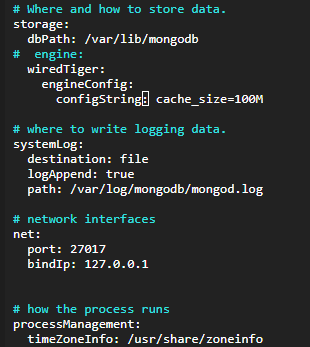
\includegraphics[scale=0.7]{figs/iu_mongod_conf.png}
    \caption{Fisierul mongod.conf}
    \label{fig:iu_mongod_conf}
\end{figure}

\subsection{Instalare programe Python}\label{subsec:iu_instalare_python}
Pentru fiecare server descris anterior exista un script python care reprezinta interfata de comunicare a server-ului. Scriptul pentru operatiile CRUD cu baza de date 
este numit "monitoring\_system\_bknd" si poate fi descarcat de la adresa \url{https://github.com/Coposescu/monitoring\_system\_bknd/tree/master}, iar scriptul 
care intercepteaza toate mesajele de la broker-ul MQTT se numeste "MQTTDataBridge" si poate fi descarcat de la adresa \url{https://github.com/Coposescu/MQTTDatabaseBridge}.

Pasii pentru instalarea programelor pe o masina cu sistem de operare linux sau windows sunt descrisi mai jos:
\begin{enumerate}
    \item Clonare proiecte de la adresele specificate mai sus in aceasta sub-sectiune.
    \item Pentru windows se instaleaza Python versiunea 3.9 de la adresa url \url{https://www.python.org/downloads/release/python-390/} (atentie la bifarea casutei 
    "Add python.exe to PATH"), iar pentru Linux prin executarea comenzii "sudo apt install python3.9".
    \item In interiorul directorului fiecarui proiect, "monitoring\_system\_bknd" si "MQTTDataBridge", se deschide un terminal (Linux) sau un "Command Prompt" (windows) si 
    se executa comanda "python -m venv .venv" pentru crearea unui mediu virtual. Acest mediu virtual trebuie activat prin executarea comenzii "source .venv/bin/activate" 
    in Linux si ".venv/Scripts/activate" in windows. 
    \item Ambele proiecte contin un fisier numit "requirements.txt". Aceste fisiere contin librariile necesare pentru executarea programelor. Pentru instalarea acestor 
    bibloteci se va executa comanda "python -m pip install requirements.txt". Inainte de executia acestei comenzi in terminalul Linux sau windows trebuie sa apara "(venv)".
    \item Pentru executarea programelor, in terminalul Linux sau in Command Prompt se executa comenzile "python run\_bridge.py" si "python run\_bknd.py".
\end{enumerate}

\section{Instalare aplicatie Android}\label{sec:iu_instalare_app_android}
Pasii pentru instalarea aplicatiei Android pe un telefon mobil cu sistem de operare Android sunt prezentati in urmatoarele puncte:
\begin{enumerate}
    \item Clonare proiect de la adresa \url{https://github.com/Coposescu/IoTApp_3}.
    \item Instalare mediu de programare Android Studio Chipmunk 2021.2.1 de la adresa \url{https://developer.android.com/studio/archive}.
    \item Dupa instalare se deschide mediul Android Studio si din meniul File -> Open se cauta directorul proiectului cu numele "IoTApp\_3" si se selecteaza "OK". La 
    incarcarea proiectului vor fi instalate automat toate bibliotecile necesare executarii proiectului (fisierul build.gradle contine aceste informatii).
    \item Pe telefonul mobil trebuie activat modul "Developer". Aceasta setare este diferita pentru fiecare telefon Android si se gaseste in manualul de utilizare al 
    acestuia.
    \item Se conecteaza telefonul mobil printr-un cablu USB la calculator si se selecteaza din telefon "Transfer Files". In scurt timp, Android Studio va detecta automat 
    telefonul.
    \item Din meniul "Run" se selecteaza "Run 'app'" si se asteapta incarcarea aplicatiei pe telefon. La final, pe telefon va aparea o iconita ca in figura 
    \ref{fig:iu_android_icon}
\end{enumerate}

Figura \ref{fig:iu_android_icon} prezinta inconita aplicatiei Android dupa instalare.
\begin{figure}[H]
    \centering
    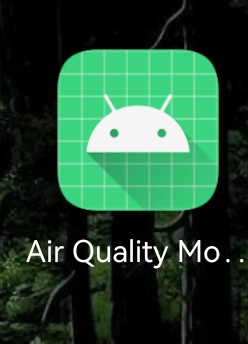
\includegraphics[scale=0.3]{figs/iu_android_icon.png}
    \caption{Inconita aplicatiei Android}
    \label{fig:iu_android_icon}
\end{figure}

\section{Utilizarea sistemului}\label{sec:iu_utilizare_sistem}
Pasii pentru prima utilizare a sistemului de monitorizare a calitatii aerului sunt enumerati mai jos:
\begin{enumerate}
    \item Alimentare senzor prin intermediul unui cablu micro USB.
    \item La prima deschidere a aplicatiei "Air Quality Monitor" ecranul va arata ca in prima captura de ecran din figura \ref{fig:iu_android_screens}.
    \item Pentru instalarea senzorului in aplicatie trebuie apasat butonul "+" din partea de jos a ecranului. Aceasta actiune va deschide o noua fereastra care va cere 
    introducerea numelui retelei Wi-Fi (SSID) si parola acesteia. Aceasta fereastra reprezinta primul pas din procesul de instalare. Prin apasarea butonului "Next" 
    se va deschide o fereastra care reprezinta pasul 2 din procesul de instalare si tot asa pana la pasul 4. Ferestrele specifice instalarii contin intructiuni text care explica 
    ce trebuie facut.
    \item Dupa finalizarea procesului de instalare ecranul aplicatiei va arata ca in a doua captura din figura \ref{fig:iu_android_screens}. In aceasta fereastra este afisata o 
    lista a senzorilor, statusul conexiunii senzorului "Connected", numele si tipul.
    \item Pentru vizualizarea valorilor transmise de catre un senzor se apasa pe numele acestuia. Noua fereastra va arata ca in a treia captura din figura 
    \ref{fig:iu_android_screens}. Tot aici sunt afisate si informatii detaliate despre senzor.
    \item Pentru vizualizarea valorilor sub forma grafica se apasa pe oricare valoare afisata in ecranul curent. Noua fereastra va arata ca in captura 4 din figura 
    \ref{fig:iu_android_screens}. Din lista din dreapta sus unde este afisat "10m" se poate selecta perioada pe care se doreste vizualizarea graficului.
    \item Pentru reinstalarea senzorului, in cazul in care se doreste conectarea acestuia la un alt router, trebuie mentinut apasat butonul "BTN0" de pe senzor (de pe 
    placa Arty Z7) timp de 5 secunde. Un LED albastru va aparea pe placa daca butonul a fost mentinut suficient. Senzorul trebuie sters din aplicatie si urmat din nou 
    procesul de instalare.
\end{enumerate}

Figura \ref{fig:iu_android_screens} prezinta inconita aplicatiei Android dupa instalare.
\begin{figure}[H]
    \centering
    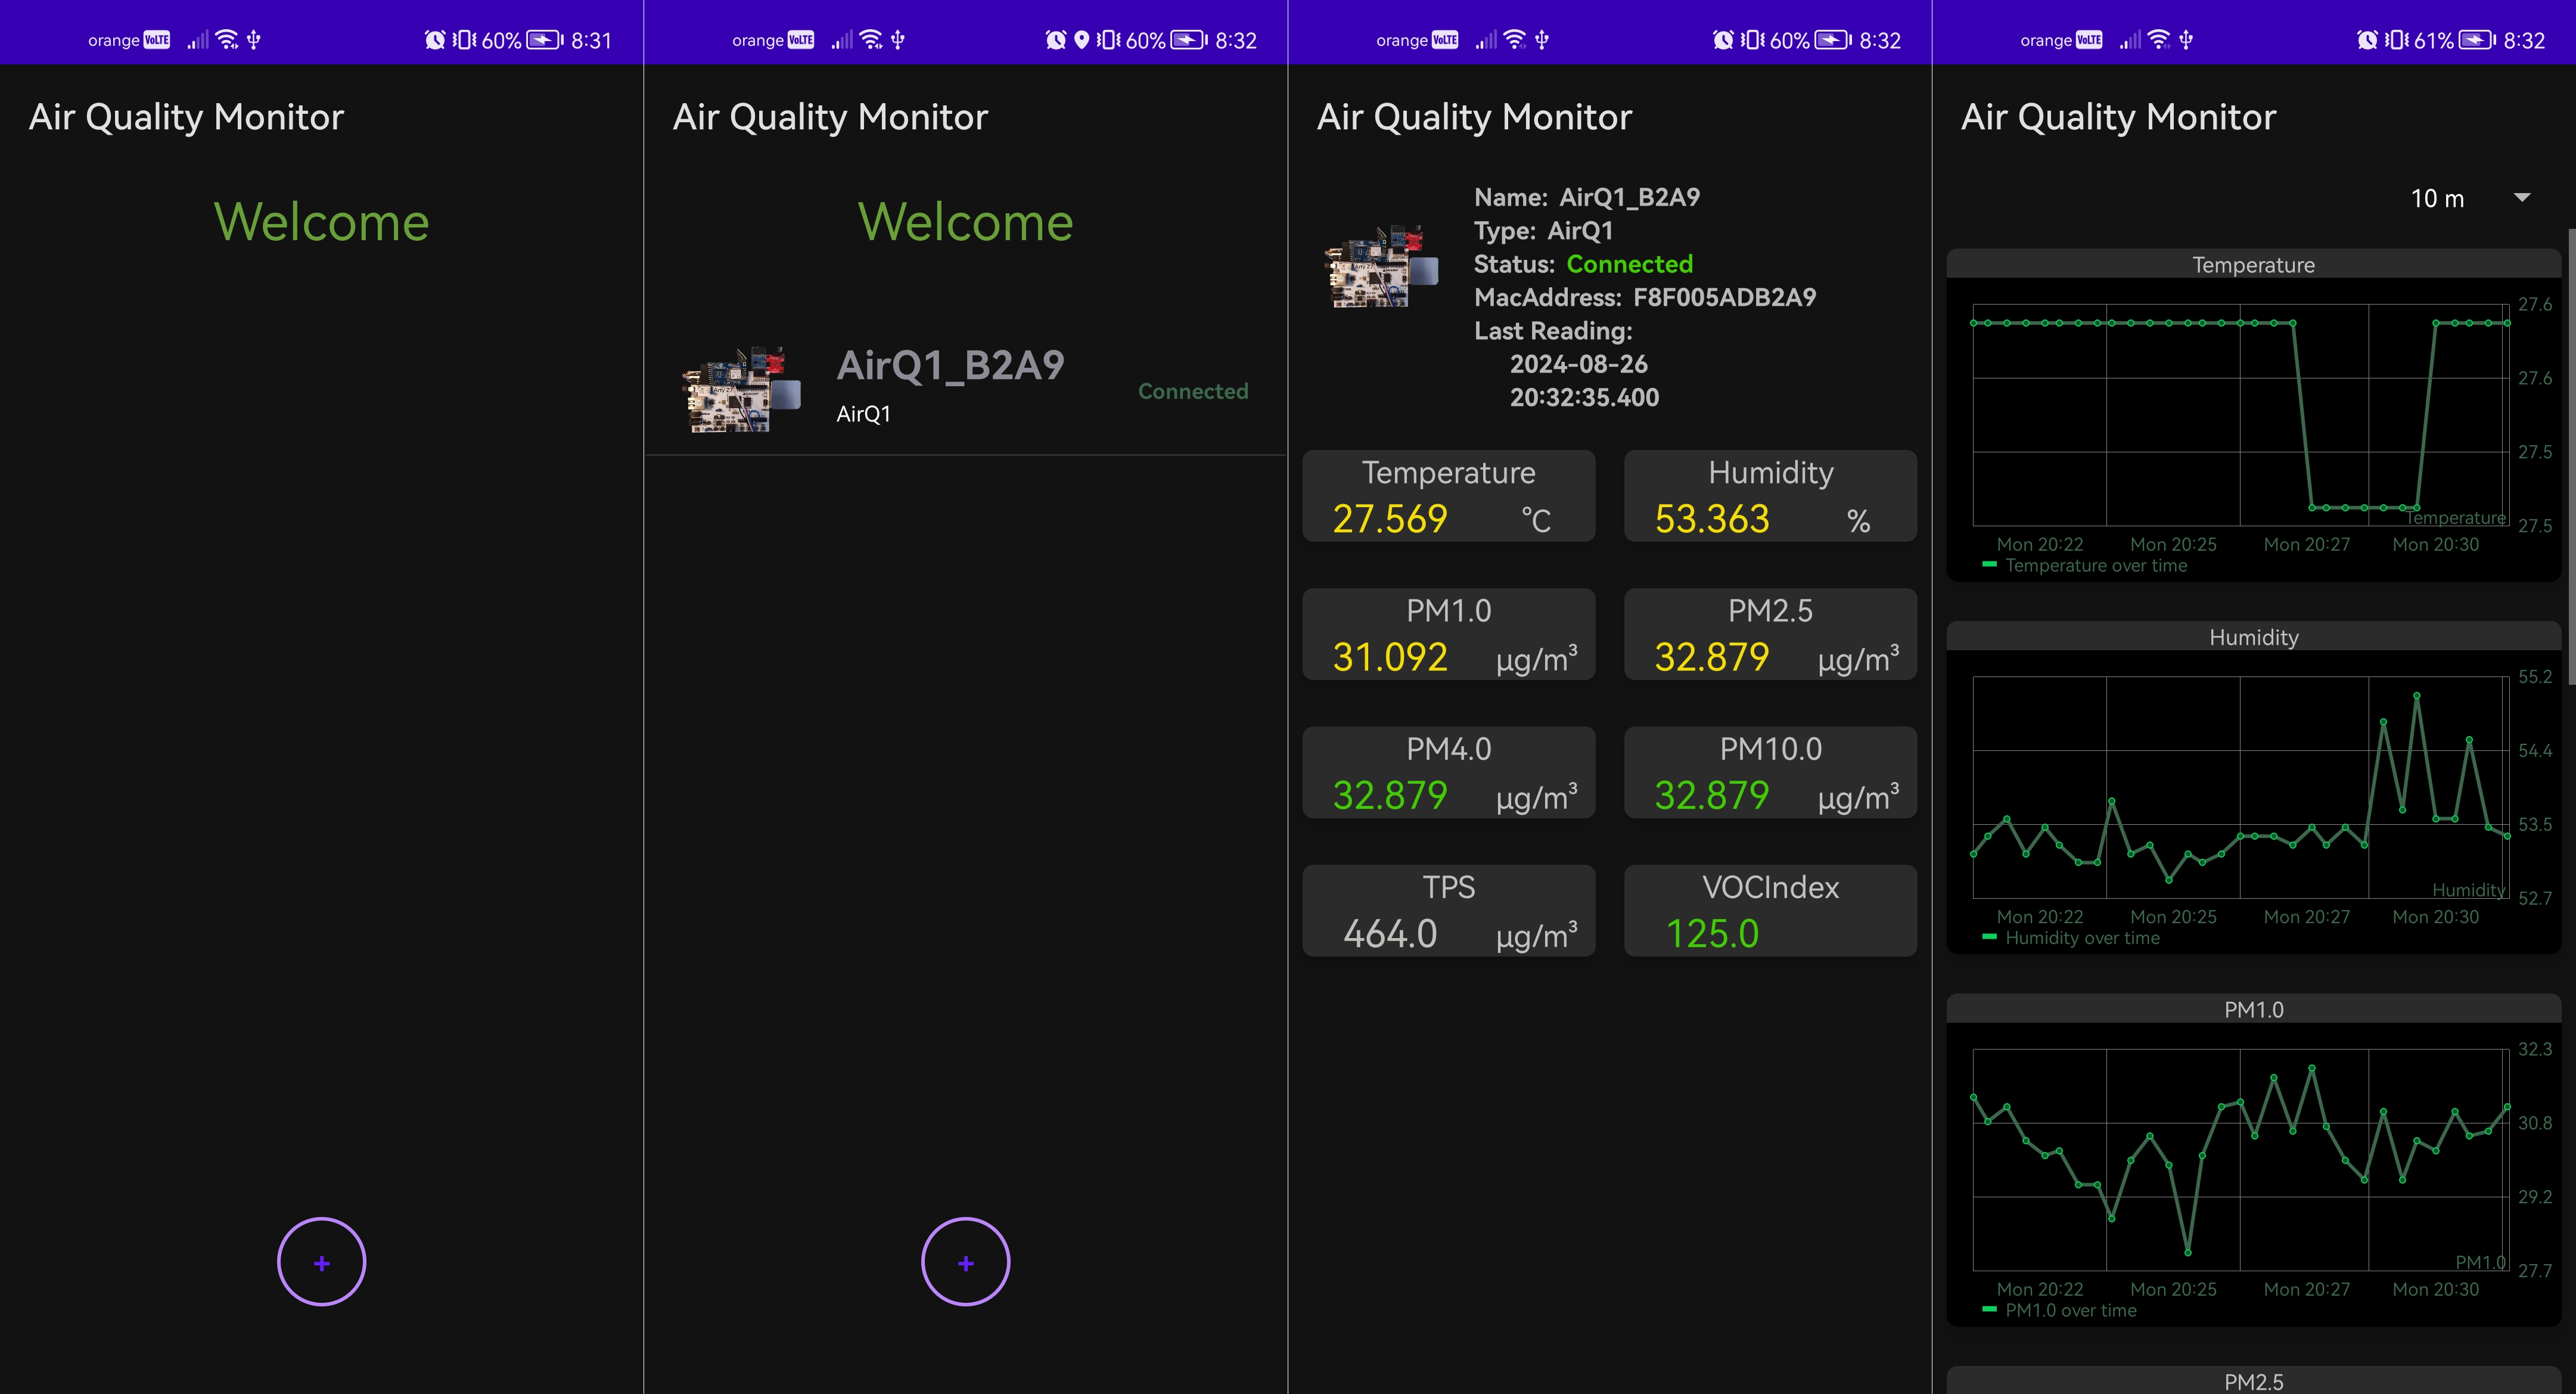
\includegraphics[scale=0.12]{figs/iu_android_screens.png}
    \caption{Capturi aplicatie Android}
    \label{fig:iu_android_screens}
\end{figure}